\section{Introducción y Alcance del Rol Individual}

\subsection{Contexto General del Proyecto ALUNA PBR-02}
El proyecto \textbf{ALUNA PBR-02} surge como una solución multidisciplinar para abordar uno de los problemas más críticos en la biotecnología marina aplicada al trópico: el sobrecalentamiento térmico en fotobiorreactores cerrados. En regiones costeras como Santa Marta (Colombia), la temperatura ambiente oscila comúnmente entre $28\,^\circ\text{C}$ y $35\,^\circ\text{C}$, y la radiación solar directa supera los $900\,\text{W/m}^2$.

La cepa objeto de cultivo, \textit{Tetraselmis chuii} (Clorofita marina flagelada de alto valor nutricional y lipídico), exige un rango operativo estricto de \textbf{$20.0\,^\circ\text{C}$ a $22.0\,^\circ\text{C}$}. Temperaturas superiores a $25\,^\circ\text{C}$ inducen fotooxidación y degradación de clorofilas, mientras que alcanzar los $35\,^\circ\text{C}$ provoca la desnaturalización enzimática y la lisis celular masiva e irreversible.

\begin{figure}[htbp]
    \centering
    \begin{subfigure}[b]{0.48\textwidth}
        \centering
        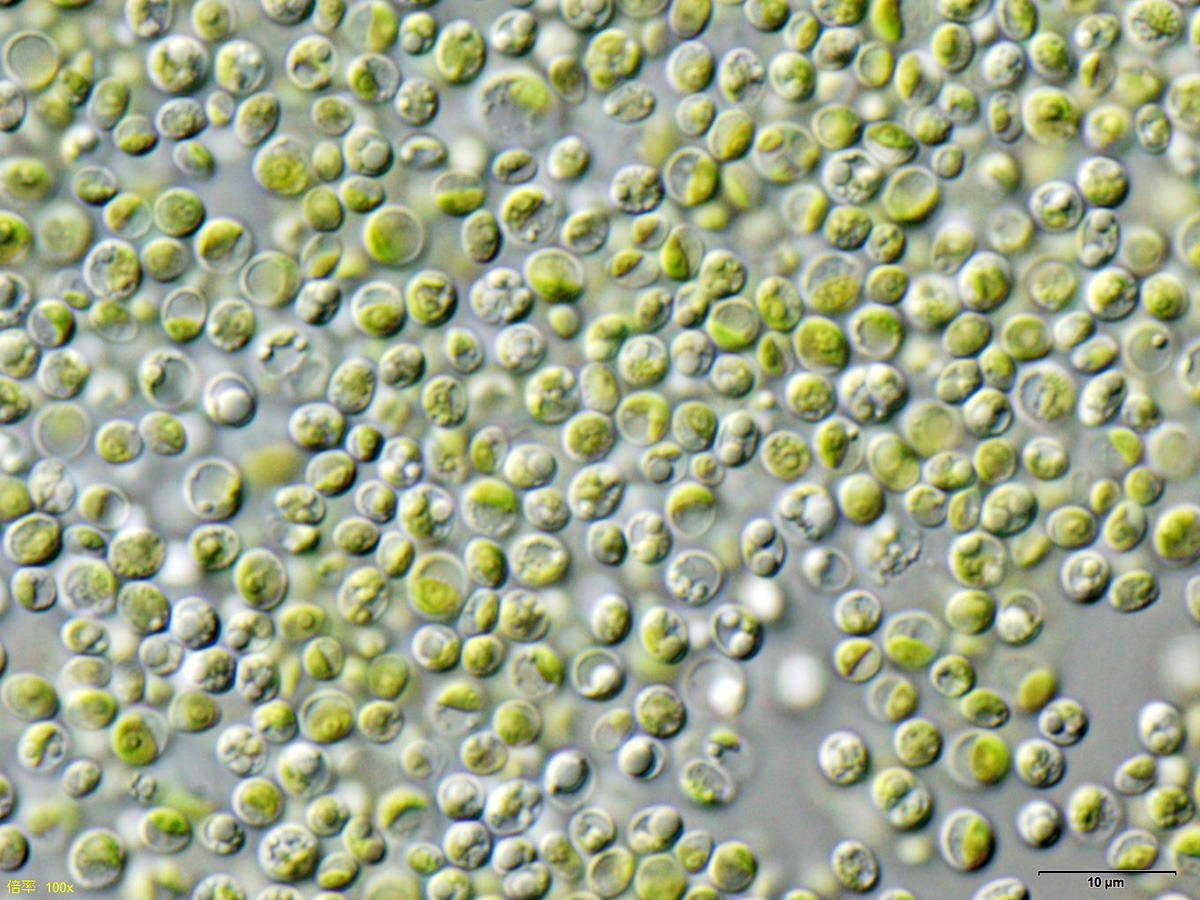
\includegraphics[width=\textwidth]{imagenes/cultivo_tetraselmis.jpeg}
        \caption{Cultivo experimental de \textit{Tetraselmis chuii}.}
        \label{fig:tetraselmis}
    \end{subfigure}
    \hfill
    \begin{subfigure}[b]{0.48\textwidth}
        \centering
        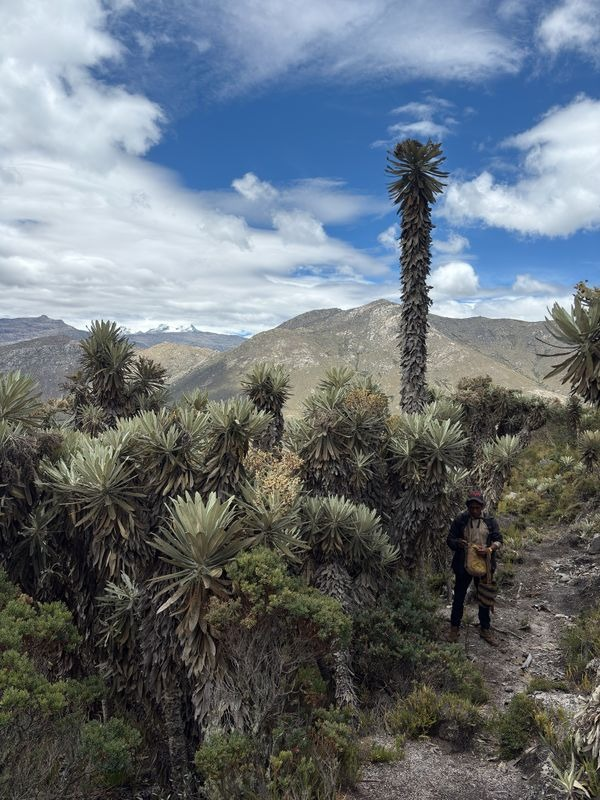
\includegraphics[width=\textwidth]{imagenes/frailejon_snsm.png}
        \caption{\textit{Espeletia occulta} en la Sierra Nevada.}
        \label{fig:frailejon}
    \end{subfigure}
    \caption{Fundamentos biológicos y biomiméticos del proyecto ALUNA PBR-02.}
    \label{fig:bio_intro}
\end{figure}

Para resolver este desafío sin recurrir a costosos e ineficientes chillers industriales (que exceden con creces los \$15'000.000 COP), se adoptó un principio de \textbf{Biomímesis con Lógica Invertida} inspirado en el Frailejón (\textit{Espeletia occulta subsp. glossophylla}), planta endémica de la Sierra Nevada de Santa Marta. Mientras el frailejón cierra sus hojas en la noche para atrapar calor frente a heladas de páramo ($<0\,^\circ\text{C}$), el biorreactor cierra un escudo textil reflectivo en horas pico para \textbf{atrapar el frío generado por una celda Peltier} y rebotar la sobrecarga radiativa del sol caribeño.

\subsection{Matriz de Responsabilidades y Alcance Individual}
En el marco del equipo de trabajo, asumí de manera autónoma la responsabilidad integral de los componentes de \textbf{modelado matemático, simulación computacional, desarrollo digital y software embebido/IoT}. Mis responsabilidades específicas comprendieron:

\begin{enumerate}[label=\textbf{\arabic*.}]
    \item \textbf{Modelado Matemático Dinámico:} Formulación matemática acoplada de la cinética biológica (Modelo de Droop) y del balance térmico diferencial con bombeo termoeléctrico (Efecto Seebeck/Peltier), pérdidas convectivas y radiación solar.
    \item \textbf{Simulación Computacional y Generación en MATLAB/Simulink:} Creación completa del entorno de simulación numérica en MATLAB y programación procedural del modelo de bloques \texttt{aluna\_pbr\_simulink.slx} mediante scripts automatizados (\texttt{crear\_modelo\_simulink.m} e \texttt{init\_simulink\_aluna.m}).
    \item \textbf{Diseño de Filtros DSP y Control Híbrido:} Parametrización en simulación de filtros digitales IIR (EMA), Promedio Móvil (MA) y filtros analógicos anti-aliasing, junto con la lógica de conmutación suave (sigmoide) para el escudo tipo Frailejón.
    \item \textbf{Firmware Embebido en ESP32 (C++):} Programación del microcontrolador para adquisición concurrente de sensores OneWire DS18B20, modulación de potencia PWM en hardware (LEDC a 1 kHz) y control servomotor en ángulo continuo.
    \item \textbf{Arquitectura Full-Stack IoT en Tiempo Real:} Implementación del backend en Python (Flask) con subprocesos de comunicación serial a 115200 baud, buffer de telemetría y desarrollo del Dashboard web reactivo en Astro, TypeScript y Apache ECharts.
    \item \textbf{Integración Eléctrica de Hardware y Puesta a Punto:} Diseño y montaje del conexionado de potencia, aislamiento de masas, acondicionamiento de señales y depuración experimental de fallas térmicas y eléctricas.
\end{enumerate}
